\documentclass[conference]{IEEEtran}
\IEEEoverridecommandlockouts
\usepackage{cite}
\usepackage{amsmath,amssymb,amsfonts}
\usepackage{algorithmic}
\usepackage{graphicx}
\usepackage{textcomp}
\usepackage{xcolor}
\usepackage{float}
\usepackage{hyperref}
\usepackage{appendix}
\usepackage{varwidth}
\usepackage{caption}
\captionsetup[figure]{labelfont=bf,justification=centering}
\captionsetup[table]{labelfont=bf,justification=centering}

\renewcommand{\labelenumi}{\arabic{enumi}.}
\renewcommand{\labelenumii}{\labelenumi\arabic{enumii} }
\def\BibTeX{{\rm B\kern-.05em{\sc i\kern-.025em b}\kern-.08em
    T\kern-.1667em\lower.7ex\hbox{E}\kern-.125emX}}
\usepackage[utf8]{inputenc}

\bibliographystyle{plain}

\title{Fighting Literature Illiteracy With Data Processing: Development of a Search System Using Book Data}

\author{
\IEEEauthorblockN{Frederico Rodrigues\IEEEauthorrefmark{1}, Mateus Silva\IEEEauthorrefmark{2} and Melissa Silva \IEEEauthorrefmark{3}}
\vspace{0.05in}
\IEEEauthorblockA{\IEEEauthorrefmark{1}FEUP. \emph{up201807626@up.pt}}
\IEEEauthorblockA{\IEEEauthorrefmark{2}FEUP. \emph{up201906232@up.pt}}
\IEEEauthorblockA{\IEEEauthorrefmark{3}FEUP. \emph{up201905076@up.pt}}
}

\date{September 2022}

\begin{document}

\maketitle

\begin{abstract}
With reading as a general theme, our data processing project intends to facilitate the finding of books for all readers with a personalized yet still efficient way to guide newcomers into this hobby, thus answering and aiding in the reduction of what's perceived as a gap in understanding most book characteristics. Statistical analysis performed on our final data set allowed us to confirm expectations we had on the data, become accustomed to it, and thus allowed for the definition of concrete information needs. Our main angle is to transform big sources of data on books into more digestible and easily navigable results for our users to find themselves fitting book recommendations.
\end{abstract}

\section{Introduction}
Reading tends to be seen as an unimportant, if not downright boring, hobby. We've heard about countless excuses or justifications for people to not read, ranging from understandable to simply false - \textit{Sure, the movie adaptation is better!} \newline
Despite this, it has been proven to be a fundamental activity: a study made by APA shows that over 80\% of teenagers don't read for leisure daily \cite{twenge2019trends}, which sounds way more serious when we add the conclusion from another study, stating that reading could help reduce mental decline in old age by up to 32\% \cite{Wilson314}. \newline
We don't intend to prove the thesis that reading should be considered a forming activity in every human's life - science already backs us up, so what we bring is a solution for the general aversion to it using work made in the context of the course unit of \textit{Information Processing and Retrieval}. \newline
This report exposes all the work made towards a solution through obtaining, exploring, and effectively utilizing book data and working it within the context of an organized and directed system. \newline
As of now, only information gotten within work made for the first project delivery is included here. We expect to include any useful details from every step of our process.

\part{Data Preparation}

\section{Data Set}
When reading was selected as a theme, we started looking for data sets in multiple open data platforms. We landed on two data sets: \textbf{'GoodReads 100k Books'} \cite{grkaggle} and an Amazon data set with book reviews. Both were found for free on Kaggle, a platform made especially for sharing data set analysis and files. \newline
The data from the first data set was retrieved by the author by scraping the Goodreads website and has \textbf{120.17 MB}. This data set includes numerical attributes such as page count and average rating and textual attributes like the book's description and its associated ISBN.  \newline
We originally wanted to use the two data sets together by joining them; however, this proved impossible since the Amazon data set identifies books by an Amazon-attributed product identifier called ASIN. We attempted scraping Amazon's website pages for the respective ISBNs only to find this wasn't available, thus we abandoned this plan and scraped data from other platforms, as explained next.

\subsection{Pipeline Characterization}
\textbf{Fig. \ref{fig:pipeline}} describes our project's pipeline in a visual diagram.\newline
The original data set was comprised of 100K rows in a table of 13 columns. We quickly noticed the raw data set was multilingual and included text in other languages and any needed accents tended to get lost due to the base encoding format the files came in. We quickly fixed this by running the files through a Windows PC's native Notepad application and saving them in ANSI encoding. We reapplied this technique whenever adequate. \newline
After this, we used OpenRefine for initial data analysis, focused on missing data. Through this, we found out Goodreads provides incomplete information on a relatively small set of books within our data set - we decided on deleting them considering the loss comprised less than one-fifth of the original data set, thus leaving us with 72.2K rows. \newline
Through further analysis, we found that some numerical attributes (page count, average rating, and review count) were sometimes filled with the value 0. Thus, we went back to Goodreads and found that a big number of these did have listed values different from 0. We used Python to scrape this information from Goodreads when we could. \newline
Meanwhile, we had an idea for our platform which would require us to use book prices, and since no platform seemed to provide an API from where we could easily get this information, we once again turned to web scraping. The winning platform proved to be Book Depository, an international online bookshop, mostly because it allowed for searching by ISBN. We consider this process moderately successful - we managed to get a price for roughly 27.4K books. \newline
All of these activities reduced our 0 values to less than 3K. However, when we saw just how successful we were in scraping Book Depository, we went back to it again, this time to try and get values for page counts, effectively reducing the last mentioned count to 2K, after which, we considered it a good number to stop at. \newline
Afterward, we found it fitting to scrape Goodreads again for reviews since the Amazon data set couldn't be used. There was an associated process of translation of many reviews that weren't written in English, for which we used Python libraries. Since most libraries had a limit for translatable text in the range of 3-5K characters, we discarded all reviews that surpassed this limit. The translation process was also applied to some of the original attributes where we discovered non-English writing. \newline
We then proceeded into some data cleaning, namely the removal of repeated space between words (book descriptions were the main offender), duplicate removal (in book genre), and normalization of the book format values. We also proceeded to remove the ISBN-13 column from the original data set as ISBN served the same purpose. \newline
Finally, we ended up with 71K rows and 13 columns, which we subjected to statistical data analysis through Python - Pandas, Seaborn, and Pyplot, for example. \newline
It's possible to recreate the entire process using this project's \textit{makefile} by using the command \textit{make all}.

\subsection{Final State of the Data Set}
\begin{figure}[h]
    \centering
    \includegraphics[height=7.5cm]{figures/UML_diagram.png}
    \caption{UML diagram for the final state of the data set.}
    \label{fig:uml}
\end{figure}

The above diagram (\textbf{Fig. \ref{fig:uml}}) visually represents our final data set.
Our final data set has three main entities: Book, Review, and Profile. The Book table merely compiles the collected attributes, from author name and title to average price and average rating. Whenever a Review is associated with a Book entry, it includes the review text and the Goodreads book page URL. The final table, Profile, is not part of our data set yet, as it is something we aim to get to - in general terms, we intend to derive a Book's Profile out of its associated Reviews. \newline
A Book Profile comprises attributes like: (plot) pacing, mood, sensitivity (in dealing with certain content warnings) and how meaningful is a book's average rating when considering the review count \footnote{To illustrate our point: a Book with a 5/5 rating possesses a higher value the higher its total rating count is.}.

\subsection{Characterization of the Final Data Set}
We made some statistical analysis of the final data set by using Python libraries, like Pandas and Seaborn. \newline
We divided our analysis into two parts: the first part comprised a more simple analysis of the data while the second part focused on trying to assess harder-to-discover qualities in our data.
For our first part, we found it useful in guiding our process by a few expectations. Here are some examples:
\begin{enumerate}
    \item Since Romance is by far the best-selling genre in fiction books, we were expecting it to rank high on a ranking of book count by genre;
        \begin{enumerate}
            \item At the same time, because of this and because the average Romance novel is around 90k words, which tends to translate into 200-400 pages, we expected our page count to be more frequent in that range;
        \end{enumerate}
    \item Though digital reading has become more popular, we were expecting printed format books to be heavily present;
    \item Knowing the raw data set collected data starting in 2017, we expected some of the mainstream fiction trends to be reflected by titles in it: for example, dystopian fantasy (i.e.: \textit{The Hunger Games} by Suzanne Collins) or contemporary young adult novels (i.e.: \textit{The Fault in Our Stars} by John Green);
        \begin{enumerate}
            \item Considering mainstream popularity we also expected titles like these to have a review count on the higher side.
        \end{enumerate}
\end{enumerate}
Most, if not all, of our expectations, proved to range from reasonably correct to completely correct. For example, we have a histogram showing the distribution of values on the data set's page count attribute see \textbf{Fig. \ref{fig:hist}}. We also studied the ten most frequent genres across their average values for numerical attributes - see \textbf{TABLE I}. \newline 
For the second part of our analysis, we focused on the deeper characteristics of the final data set. We wanted to see how certain attributes interacted with each other, thus we did a heat map graph of the correlation measures between all of the book data numerical attributes - see \textbf{Fig. \ref{fig:heatmap}}.
We finished this analysis with a way higher familiarity with our data set and higher confidence in its data since it did confirm our expectations.

\subsection{Information Needs}
Since our perception and liking of reading for leisure might prove itself to be a biased starting point, this section hopes to shine a light on why we chose to do this work, why we consider the work we present needed, and what our work is directed towards. \newline
If what’s being said on the page right now is being understood by someone, it means they’re reading. From here, we’d like to direct the reader’s attention to why they’re reading. Is it because our title was catchy? Because our abstract was enticing? Because someone needs to read this for us to get a grade? \newline
By answering that, we’re on the right track to understanding why a general aversion to reading is so rampant. As an example, there’s been a decrease in reading for leisure of around 10\% across most age groups in the past 15 years in the United States of America \cite{washingtonpost}. \newline
We attribute these worrisome results to the way most people experience reading. Every single person who's gone through some part of an education system has inevitably been faced with a reading assignment on a book: in America, it might be \textit{Catcher in The Rye}, in Portugal, \textit{Memorial do Convento}. Reading by force turns the activity into a chore - and when something’s labeled a chore, we'll do anything to avoid it. \newline
This turns reading into something foreign, a barrier very rarely surpassed by literature we'd call, at best, dubious - i.e., celebrity autobiographies. \newline
Fixing these problems at the root is beyond the scope of what we've learned in \textit{PRI} classes, so our main objective is to fight what we call \textbf{\textit{literature illiteracy}}. We define it as a \textit{general lack of knowledge about the characteristics of books, namely: pacing, genre, popular opinion, and sensitivity}.  \newline
Our data set and solution intends to make searching for books and getting good recommendations to start as easy and enjoyable as possible, hence the following information needs, starting with a general main question from which we intend to augment the specificity.
    \begin{enumerate}
        \item \textbf{Main Question:} \textit{How to give a transparent and corroborated sense of a book's content and alignment with personalized interests to a user looking for their next book to read?}
    \begin{enumerate}
        \item \textit{Search by Buzzwords}: we intend to let users search by suggested buzzwords that occur in reviews which are then associated with the corresponding books; 
        \item \textit{Search by Book Profile}: through our Book Profiles, we intend to let users search by pre-made, easily understandable terms that characterize books in a corroborated manner;
        \item \textit{Traditional Filterable Search}: we intend to let our users search by a book's associated attributes through filters included on our search engine - for example: search by author name, ISBN, rating range, book format, et cetera;
        \item \textit{Matchmaking by Similarity}: we intend to let our users search for similar books to a certain entry, once again by providing statistics on the matching of Book Profiles (for example, \textit{50\% match}).
    \end{enumerate}
\end{enumerate}

\section{Conclusion}
We finish this first part of the work with a data set we believe is ready for our planned uses in the future. As shown, our data set is substantial and we've also shown some of our data set's range through statistical analysis, which gives us confidence in using this data set in the future. \newline
Considering our objective, we proposed adequate information needs to provide a pleasing experience to our users and facilitate the finding of book recommendations or just book characteristics in general. \newline
With all of this in mind, our next step is to make an information retrieval system where we use this data. Besides this, we also aim to use Natural Language Processing techniques for the processing of our textual attributes and making of Book Profiles, which we see as the basis for most of our Information Needs.

\bibliography{refs}

\begin{figure}[hbt!]
    \makebox[\textwidth][c]{
    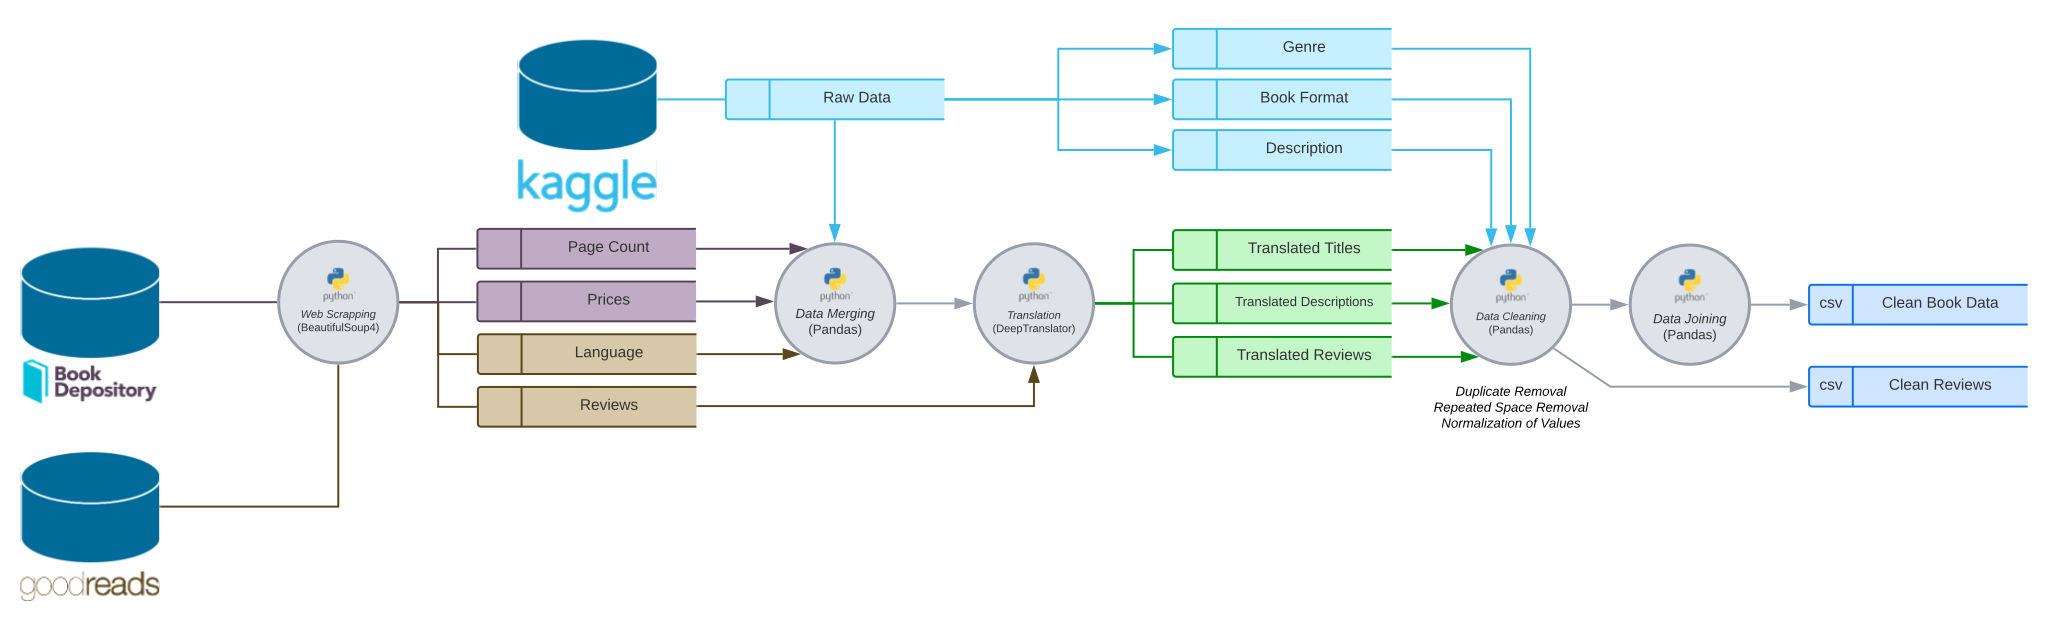
\includegraphics[width=1.15\textwidth]{figures/pipeline_diagram.png}
    }
    \begin{varwidth}{\textwidth}
        \caption{Pipeline diagram.}
        \label{fig:pipeline}
    \end{varwidth}
\end{figure}

\begin{figure}[hbt!]
\centering
\begin{minipage}{.5\textwidth}
  \centering
  \includegraphics[width=7cm]{figures/hist.png}
  \caption{Page count histogram.}
  \label{fig:hist}
\end{minipage}%
\begin{minipage}{.5\textwidth}
  \centering
  \includegraphics[width=7cm]{figures/heatmap.png}
  \caption{Numerical attributes correlation heat nap.}
  \label{fig:heatmap}
\end{minipage}
\end{figure}

\begin{table}[hbt!]
    \begin{varwidth}{\textwidth}
        \caption{Average value for numerical attributes for 10 most common genres.}
        \label{table:avg_top10}
    \end{varwidth}
    \resizebox{\textwidth}{!}{
    \begin{tabular}{ccccc}
        \textbf{Genre} &
        \multicolumn{1}{l}{\textbf{Average Rating}} &
        \multicolumn{1}{l}{\textbf{Average Rating Count}} &
        \multicolumn{1}{l}{\textbf{Average Review Count}} &
        \multicolumn{1}{l}{\textbf{Average Page Count}} \\
            Nonfiction   & 3.95 & 1439 & 100 & 301 \\
            Fiction      & 3.86 & 8056 & 476 & 276 \\
            Romance      & 3.85 & 6657 & 441 & 279 \\
            History      & 3.93 & 1283 & 94  & 333 \\
            Fantasy      & 3.90 & 9207 & 490 & 275 \\
            Cultural     & 3.88 & 2651 & 204 & 291 \\
            Historical   & 3.86 & 5269 & 365 & 325 \\
            Literature   & 3.87 & 6093 & 317 & 313 \\
            Childrens    & 3.92 & 4376 & 219 & 122 \\
            Contemporary & 3.79 & 8648 & 623 & 276
    \end{tabular}
    }
\end{table}



\end{document}
